\documentclass[a4paper]{clase_fiuba}
\newcommand{\codigoMateria}{86.05}
\newcommand{\nombreMateria}{Señales y Sistemas}

\newcommand{\numeroTP}{1}
\newcommand{\descripcionTP}{Detección de latidos cardíacos}
\newcommand{\tituloTP}{Trabajo Práctico n°1}
\newcommand{\facultad}{Facultad de Ingeniería}
\newcommand{\universidad}{Universidad de Buenos Aires}
\newcommand{\cuatrimestre}{2° Cuatrimestre de 2017}

\usepackage{estilo_fiuba}

% ---------------------------------------------------------------
% Inicio documento
\begin{document}
\nocite{*}
% ---------------------------------------------------------------
% Caratula e índice
%******************************************************
%* Santiago Roman (FIUBA #93947)
%******************************************************
% Estilo de la caratula
% -----------------------------------------------------

  \thispagestyle{empty}
  \newgeometry{twoside, left=2.5cm,top=2cm,right=2.5cm,bottom=1.5cm,bindingoffset=.5cm}
  \begin{titlepage}

      \centering
      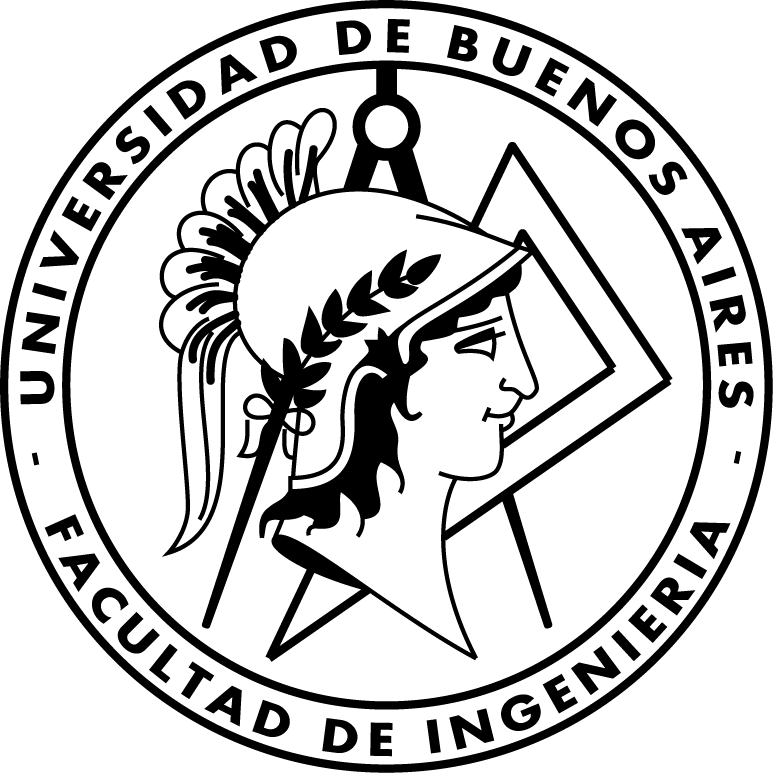
\includegraphics[scale = 0.75]{images/logo_fiuba.png}\\[1.0 cm]	% Logo universidad
      \textsc{\LARGE \universidad}\\[0.5 cm]	% Nombre universidad
      \textsc{\Large \facultad}\\[2.0 cm]	% Facultad
      \textsc{\Large \cuatrimestre}\\[2.0 cm]	% Cuatrimestre
      \textsc{\Large \codigoMateria}\\[0.5 cm] % Código materia
      \textsc{\large \nombreMateria}\\[0.5 cm] % Nombre materia
      \rule{\linewidth}{0.2 mm} \\[0.4 cm]
      { \huge \tituloTP}\\[0.5cm]
      { \huge \bfseries \descripcionTP}\\
      \rule{\linewidth}{0.2 mm} \\[1.5 cm]

       \begin{minipage}{0.5\textwidth}
           %\large{ Grupo 10}
          \begin{flushleft} \large
              \emph{Integrantes:}\\
          \end{flushleft}
      \end{minipage}~
      \begin{minipage}{0.4\textwidth}
          \begin{flushright} \large
              \emph{Padrón:} \\
          \end{flushright}
      \end{minipage}\\

      % Agregar aqui los integrantes del trabajo
      \teammember{Sanchez, Marcelo}{87685}{marce\_chez@msn.com}
      \teammember{Zec, Jeremias}{92444}{jeremiaszec@gmail.com}
      \teammember{Russo, Nicolas}{93211}{nicolasrusso291@gmail.com}
      \teammember{Garcias, Ezequiel}{93191}{garciaezequiel91@gmail.com}

      \vfill

      {\large \today}\\[2 cm]

      \vfill

  \end{titlepage}
  \restoregeometry
\thispagestyle{empty}
\clearpage

\pagenumbering{Roman}

\tableofcontents

% ---------------------------------------------------------------
% Cuerpo del informe.
\pagenumbering{arabic}
\pagestyle{fancy}
\newpage
\section{Objetivos}
\label{sec:obj}

El objetivo del presente trabajo es, en primer lugar, realizar un análisis en tiempo y
frecuencia de la señal FPG obtenida a partir de la grabación de video de un smartphone.
Posteriormente, se implementará una serie de filtros para obtener la componente "AC" de la
señal, la cual se utilizará finalmente durante la implementación del detector de latidos. En
lugar de utilizar el video directamente como señal, lo cual resulta demandante con la
memoria, se trabajará con las intensidades de color para cada frame del video en cuestión.

%\newpage
\section{Enunciado}
\label{sec:enun}
\textbf{Detección de latidos cardíacos.}
\textbf{1.} Cargar el archivo intensidad_RGB.mat y visualizar la señal RGB en
superposición (3 canales). Elija alguno de los 3 canales que, según su criterio, posea
la señal más útil a los efectos de analizar la dinámica de los latidos y utilícelo para
realizar los puntos siguientes.\\
\textbf{2.} Del gráfico del punto anterior, estimar aproximadamente los latidos por minuto
(LPM). Identifique el momento a partir del cual la frecuencia cardiaca comienza a
incrementarse, y en cuánto se incrementa.\\
\textbf{3.} Rehacer el punto anterior, pero utilizando DFT. ¿Puede en este caso identificar
cuándo se da el cambio de LPM?\\
\textbf{4.} Diseñar un filtro pasa-banda tipo Butterworth con banda de paso entre 0.5 Hz y 10
Hz. Graficar respuesta en frecuencia (módulo y fase), diagrama de polos y ceros y
respuesta al impulso (sugerencia: usar las funciones butter y fvtool de Matlab).\\
¿Qué papel juega el orden del filtro seleccionado en su diseño?\\
\textbf{5.} Filtrar la señal FPG utilizando el filtro diseñado en el punto anterior mediante la
función filter. Grafique en superposición la señal original con la filtrada y
comente acerca de:\\
a. Remoción de derivas\\
b. Cambios en la forma de la señal\\
c. Retardo de la señal filtrada respecto de la original\\
\textbf{6.} A partir de la respuesta en fase del filtro, calcule su retardo temporal y compare con
lo observado en el punto 5c.\\
\textbf{7.} Implementar un filtrado IIR ida y vuelta para anular la fase del filtro (puede utilizar
la función filtfilt de Matlab). Justificar teóricamente el funcionamiento de este
tipo de filtrado y cuál resulta su ventaja. Filtrar nuevamente la señal FPG y comparar
el resultado con lo obtenido en el punto anterior, particularmente en la forma de la
señal y su retardo.\\
\textbf{8.} Realizar un espectrograma de la señal antes y después de filtrar, mediante la función
spectrogram de Matlab (sugerencia: utilice la función caxis para saturar los
colores del espectrograma y lograr una mejor visualización). Justificar la longitud de
ventana elegida y comente acerca del resultado obtenido, relacionándolo con los
puntos 2 y 3. Calcule la resolución en frecuencia de la ventana mediante DFT en
Matlab. ¿Cómo haría para obtener mejor resolución en frecuencia y qué se pierde con
esto?\\
\textbf{9.} Identificar en el espectrograma la zona donde el pulso se acelera. Observar con
detenimiento los componentes de frecuencia que posee la señal y justificar el origen
de cada uno (para esto último, necesitará hacer uso de la señal audio_det.mat
para explicar todos los componentes observados).\\
\textbf{10.} Realizar un detector automático de latidos. El mismo debe tomar como entrada la
señal FPG y producir como salida un vector de tiempos, donde cada tiempo
corresponde a la detección de un latido en la señal. Para esto, se sugiere implementar
los siguientes pasos:\\
a. Filtrado pasa-banda de la señal, utilizando el filtrado del ejercicio 7.\\
b. Filtro de derivada, implementado con un filtro FIR h(n)=[-2 -1 0 1 2].\\
c. Normalización con energía instantánea: primero calcular la energía
instantánea de la señal mediante un filtro MA1 de la señal del punto 10a
elevada al cuadrado; luego dividir la señal del punto b por el vector obtenido.
Esto tiene como objeto reducir el impacto de la presión sanguínea sobre el
nivel de señal.\\
d. Sobre-muestreo en un factor 4 para obtener mayor resolución temporal:
implemente el sobre-muestreo utilizando la función upsample y diseñe un
filtro interpolador FIR utilizando la herramienta fdatool de Matlab.
Grafique: respuesta en frecuencia del filtro en módulo y fase, y señal original
y sobre-muestreada en superposición.\\
e. Detector de picos mediante umbral (puede definir como umbral un valor
arbitrario).\\
f. Gráfico en superposición de la señal con las marcas de los picos detectados.
Sugerencia para el punto e: en general, un pico en la señal producirá la detección de
múltiples muestras por encima del umbral. Para reducirlas a sólo una, puede utilizar
la función diff para evaluar la primera derivada sobre el vector de muestras
detectadas (la cual contiene sólo unos y ceros), quedándose solo con las muestras
positivas que resulten y buscando, para cada una de estas, la posición del máximo
inmediato de la señal original dentro de un intervalo pre-establecido (este deberá
contener mínimamente a la duración aproximada de los picos).\\
\textbf{11.} En base a los resultados del punto anterior, calcule y grafique el intervalo temporal
instantáneo entre latidos (IBI: inter-beat interval) y los LPM instantáneos.\\
\textbf{12.} Opcional. Mejorar el detector de latidos aplicando las reglas de [5]:\\
a. Establecer como regla que, si dos latidos se detectaron con una separación
temporal menor a 200ms, sobrevive sólo aquel que corresponda al pico de la
señal mayor entre ambos.\\
b. Establecer como regla que si el IBI instantáneo aumenta repentinamente en al
menos 1.5 veces entre muestras consecutivas, puede haberse perdido la
detección de un latido. Cuando este sea el caso, realice una nueva detección
de picos dentro del intervalo correspondiente, utilizando un umbral la mitad
del nominal. Si de esta manera se halla un nuevo pico, distanciado al menos
360ms de la detección precedente, entonces clasificarlo como latido.\\
\textbf{13.} Opcional. Obtener su propia señal FPG mediante la cámara de su celular y aplicar los
análisis y algoritmos desarrollados a esta señal. Para esto, realice una grabación tal
como se explicó en la sección 1 y utilice los scripts auxiliares de Matlab para extraer
los archivos de intensidades y audio del video. Nota: para un mejor resultado en la
señal registrada, utilizar el dedo índice aplicando una leve presión sobre la lente,
evitando resultar excesivamente suave o fuerte.\\

\newpage
\section{Desarrollo}
\subsection{Ejercicios}
\label{sec:desar}
\textbf{Ejercicio 1.}

Del diagrama de la figura \ref{fig:esquemas}:

\begin{equation}
X_i = Y_{i-1}\cdot G_{i}\\
Y_{i-1} = h \cdot X_{i-1} + W_{i-1}
\end{equation}

\begin{equation}
\hspace{-4.3cm} [Y_{i-1}] = VAR [h \cdot X_{i-1} + W_{i-1}]
\end{equation}
\begin{equation*}
\hspace{2cm} = h^2 \cdot VAR [X_{i-1}] + 2COV[X_{i-1}, W_{i-1}] + VAR [W_{i-1}]
\end{equation*}

Por ser $X$ y $W$ independientes $COV[X_{i-1}, W_{i-1}] = 0$ . Queda entonces:

\begin{equation}
VAR[Y_{i-1}] = h^2 \cdot A^2 + \sigma_w^2
\end{equation}
\begin{equation}
VAR [X_i] = VAR [G_{i} \cdot Y_{i-1}] = G_{i}^2 \cdot (h^2 \cdot A^2 + \sigma_w^2)
\end{equation} 

Se pide que $VAR[X_i] = \epsilon$ . Por lo tanto:

\begin{equation}
G_{i}  = \sqrt{ \frac{\epsilon}{(h^2 \cdot \epsilon + \sigma_w^2)}}  \hspace{1cm} con \; i = 3,4....n
\label{equ:gi}
\end{equation}

Luego para el repetidor $G_2$ :

\begin{equation}
G_{2}  = \sqrt{ \frac{\epsilon}{(h^2 \cdot A^2 + \sigma_w^2)}} 
\end{equation}

Eligiendo $G_2 = G_3 = G_4 =...=G_n$, resulta $A^2 = \epsilon$
$\hspace{0.5 cm} \Longrightarrow$ \fbox{$A = \sqrt{\epsilon}$}\\

\hfill

Para expresar las ganancias en función a la relación señal a ruido (SNR). Se parte de la ecuación \ref{equ:gi}:

\begin{equation}
G_{i}  = \sqrt{ \frac{\epsilon}{(h^2 \cdot \epsilon + \sigma_w^2)}} = \sqrt{ \frac{\epsilon}{\sigma_w^2\cdot (\frac{h^2 \cdot \epsilon}{\sigma_w^2}+ 1)}} 
\label{equ:gi_2}
\end{equation}

Reemplazando por la definición SNR (ecuación \ref{equ:snr}).

\begin{equation}
G_{i}  = \sqrt{ \frac{SNR}{h^2\cdot (SNR + 1)}} 
\label{equ:gi_snr}
\end{equation}

\hfill

\textbf{Ejercicio 2.}\\

\textbf{2.1}. Escribimos las señales $Y_n$ en función de los bloques anteriores:\\

$Y_1 = X_1 h + W_1 ;\hspace{0.5 cm} X_2 = Y_1 G_2$

$Y_2 = X_2\cdot h + W_2 = (X_1\cdot h + W_1)\cdot G_2\cdot h + W_2$

$Y_2 = X_1\cdot G_2\cdot h^2 + W_1\cdot G_2\cdot h + W_2$

$Y_3 = (X_1\cdot G_2\cdot h^2 + W_1\cdot G_2\cdot h + W_2)\cdot G_3\cdot h + W_3$

$Y_3 = X_1\cdot G_2\cdot G_3 \cdot h^3 + W_1\cdot G_2\cdot G_3 \cdot h^2 + W_2\cdot G_3\cdot h + W_3$\\

$Y_n = X_1\cdot (\prod_{k=2}^nG_k)\cdot h^n + \sum_{i=1}^{n-1} [(W_i\cdot \prod_{j=i+1}^n G_j)\cdot h^{n-i}] + W_n$\\

Como $W_i$ Son iid y definimos $G_2 = G_3 =...= G_n = G$, resulta:\\

$Y_n =  X_1\cdot (Gh)^{n-1}\cdot h^n + \sum_{i=1}^{n-1} (Gh)^{n-i}\cdot W + W$

$Y_n =  X_1\cdot (Gh)^{n-1}\cdot h^n + \sum_{i=1}^n (Gh)^{n-i}\cdot W$\\

\fbox{$Y_n =  X_1\cdot (Gh)^{n-1}\cdot h^n + \sum_{i=0}^{n-1} (Gh)^i\cdot W$}\\


Denotando $N_i$ al término dentro de la sumatoria, es la variable aleatoria W escalada por una constante, y se distribuye como:\\

$N_i \sim \mathcal{N}(0, (Gh)^{2i}\cdot \sigma_W^2)$\\

Por lo tanto el término asociado al ruido se distribuye como:\\

$N_n \sim \mathcal{N}(0, \sum_{i=0}^{n-1} (Gh)^{2i}\cdot \sigma_W^2)$\\

\hfill

\textbf{2.2}. Calculamos la Varianza de la señal:\\

$VAR[X_1\cdot (Gh)^{n-1}\cdot h^n] = ((Gh)^{n-1}\cdot h^n)^2\cdot VAR[X_1] = ((Gh)^{n-1}\cdot h^n)^2\cdot A^2$

$\epsilon_{senial} = (Gh)^{2(n-1)}\cdot h^{2n}\cdot A^2$\\

Por definición: $SNR = \frac{\epsilon_{senial}}{\epsilon_{ruido}}$\\

\begin{equation}
SNR_{Y_n} = \frac{(Gh)^{2(n-1)}\cdot h^{2n}\cdot A^2}{\sigma_W^2\cdot \sum_{i=0}^{n-1} (Gh)^{2i}}
\label{equ:snr_yn}
\end{equation}

\hfill

\textbf{2.3}. Suponemos $X = A$. Reescribimos $Y_n$:\\

$Y_n = N_n + A\cdot (Gh)^{n-1}\cdot h^n$\\

Por lo tanto $Y_n \sim \mathcal{N}(\mu = A\cdot (Gh)^{n-1}\cdot h^n , \sigma^2 = \sigma_W^2\cdot \sum_{i=0}^{n-1} (Gh)^{2i}$\\

La probabilidad de error se calcula como:\\

\begin{equation*}
P_{e|X_1 = A} = P(Y_n < 0 | X_1 = A) = P(N_n + A\cdot (Gh)^{n-1}\cdot h^n < 0)
\end{equation*}

\begin{equation}
P_{e|X_1 = A} = P(\frac{-N_n}{\sqrt[]{VAR[N_n]}} > \frac{A\cdot (Gh)^{n-1}\cdot h^n}{\sqrt[]{VAR[N_n]}}) = Q(\frac{A\cdot (Gh)^{n-1}\cdot h^n}{\sqrt[]{VAR[N_n]}})
\label{equ:probe}
\end{equation}

Reemplazando la ecuación \ref{equ:snr_yn} en \ref{equ:probe}, la probalidad de error se puede calcular:

\begin{equation}
P_{e|X_1 = A} = Q(\sqrt[]{SNR_{Y_n}})
\end{equation}

Por simetría, probabilidad total (Ecuación \ref{equ:prob_tot}) y dado que $P(X_1=A) = P(X_1=-A) = 1/2$\\

\begin{equation}
P_{e,n}^a = Q(\sqrt[]{SNR_{Y_n}})
\end{equation}


\hfill

\textbf{Ejercicio 3.}

\begin{figure}[H]
  \centering
  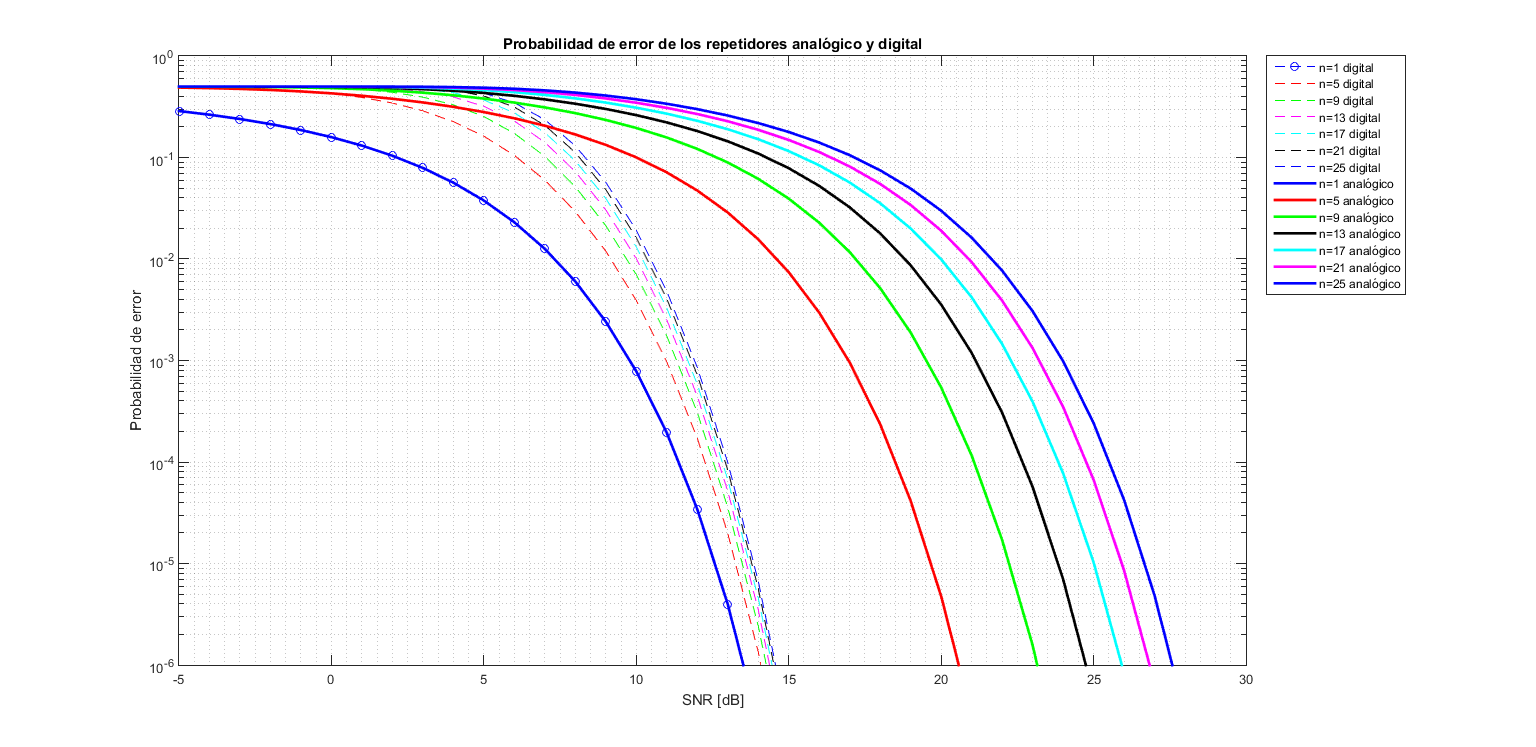
\includegraphics[width=1\textwidth]{images/Pe_pto3_1}
  \caption{Probabilidad de error de ambos sistemas con diferentes parámetros de SNR y número de etapas (n).}
  \label{fig:pto3_1}
\end{figure}

\hfill

De la figura \ref{fig:pto3_1} vemos que para cada $n$ ambos sistemas coinciden en un valor de SNR, los valores son los siguientes:

\begin{itemize}
\item 5 a -0.4 dB.
\item 9 a 0.4 dB.
\item 13 a 0.6 dB.
\item 17 a 1 dB.
\item 21 a 1.1 dB.
\item 25 a 1.2 dB.
\end{itemize}

Para cualquier número $n$ de etapas se repite el mismo comportamiento. Hasta la igualdad, ambos sistemas tienen una relación $SNR-P_e$ similar (casi idénticas). Luego de la misma, el sistema digital tiene una disminución significativamente más rápida con el aumento de la SNR.\\

Por lo tanto, conociendo el rango de SNR con el que se va a trabajar, la mejor opción es el sistema digital respecto de la Probabilidad de error en un amplio rango de valores.\\
Si el dato con el que se cuenta es la cantidad de etapas $n$, nuevamente el sistema digital es el más eficiente. En ambos casos cuando se supere ese ``umbral'' en el que ambos sistemas se comportan de manera similar.




\textbf{Ejercicio 4.}

\textbf{4.1}. Simulación de Montecarlo.

Realizamos una simulación sobre los valores de SNR dentro del intervalo  [5, 25] en dB.

Por cada valor del SNR se simularon N = 20000 veces para obtener un resultado ``óptimo´´, o sea, que los resultados concuerden con los cálculos teóricos. Los que se pueden ver claramente en las figuras \ref{fig:pto4_1} y \ref{fig:pto4_2}

\begin{figure}[H]
  \centering
  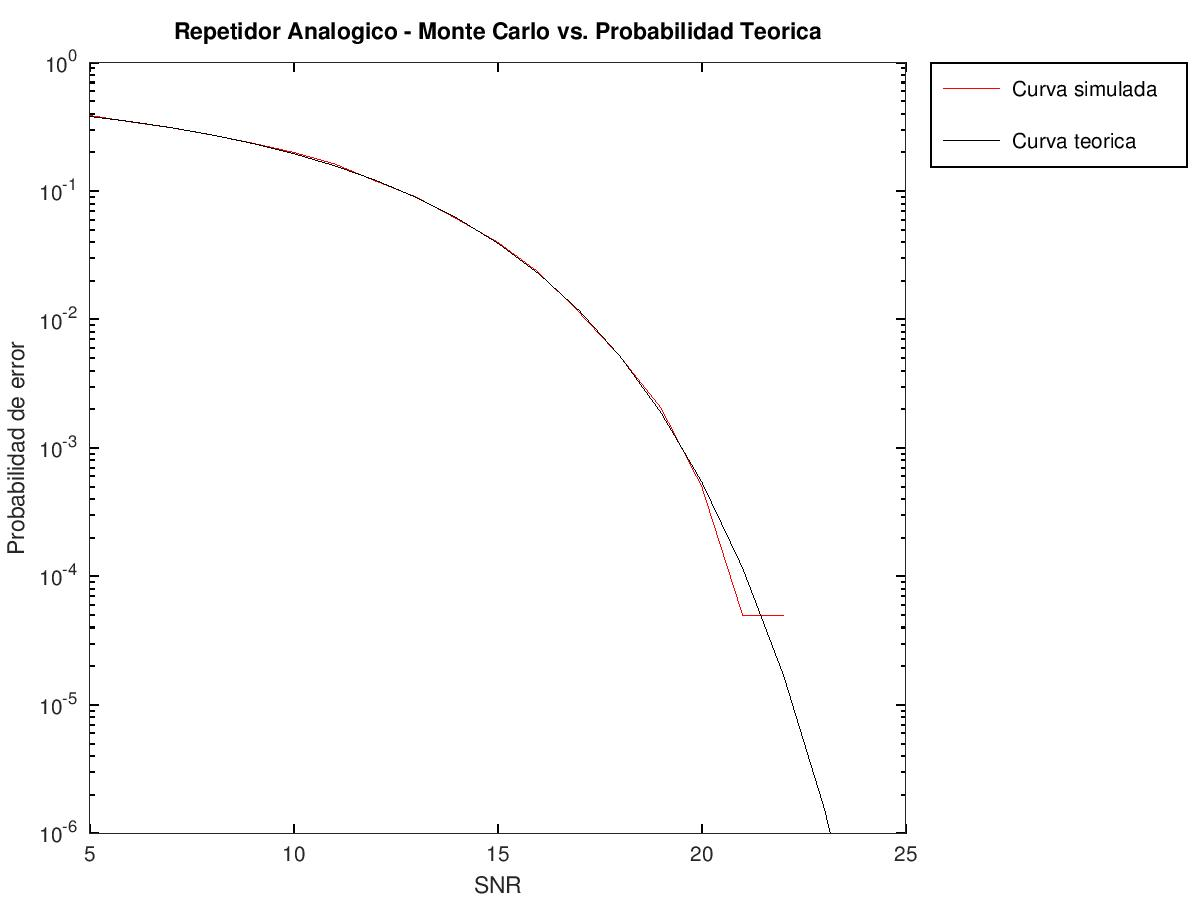
\includegraphics[width=1\textwidth]{images/Pe_pto4_1}
  \caption{Simulación de MonteCarlo para etapa analógica.}
  \label{fig:pto4_1}
\end{figure}

\begin{figure}[H]
  \centering
  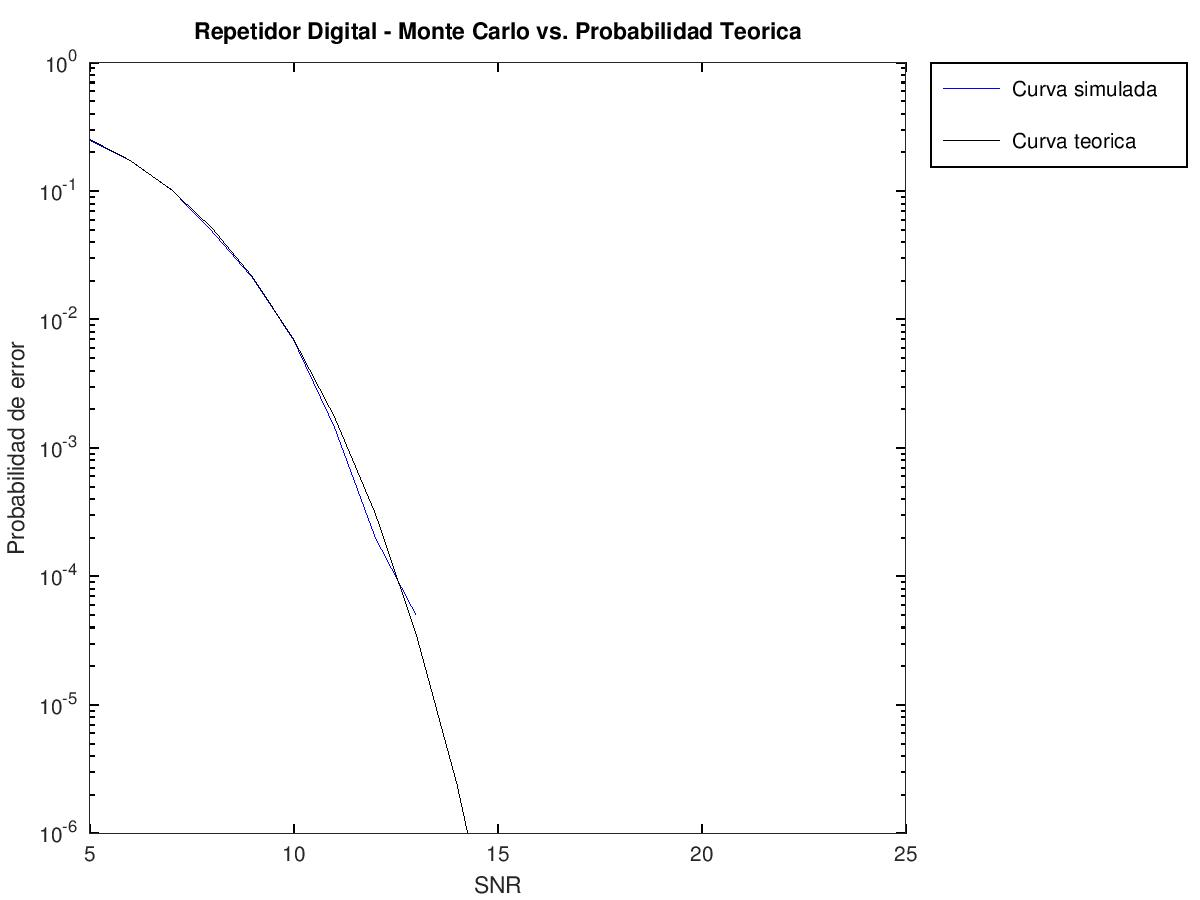
\includegraphics[width=1\textwidth]{images/Pe_pto4_2}
  \caption{Simulación de MonteCarlo para etapa digital.}
  \label{fig:pto4_2}
\end{figure}


\textbf{4.2}. Curvas de probabilidad.

Por un lado se simuló el circuito y por otro lado se propuso un modelo porbabilistico a priori que suponemos va a ajustar a nuestro circuito.
Por medio del resultado se verifica, al ver que las curvas son tan próximas, que el modelo propuesto es válido para representar el modelo real.
Se ve claramente que las curvas que se obtuvieron en la simulación se aproximan a las teóricas calculadas anteriormente. Esto se debe a que se hicieron las simulaciones ``correctamente''. Las realizaciones son efectivamente independientes. 

\newpage
%Los resultados confirman al encontrarse tan cercanos unos del otro lo calculado en la parte teórica, debido a la gran cantidad de simulaciones.

\textbf{4.3} Densidades de probabilidad de $Y_n$ (justo antes del detector) en el sistema analógico.

\begin{figure}[H]
  \centering
  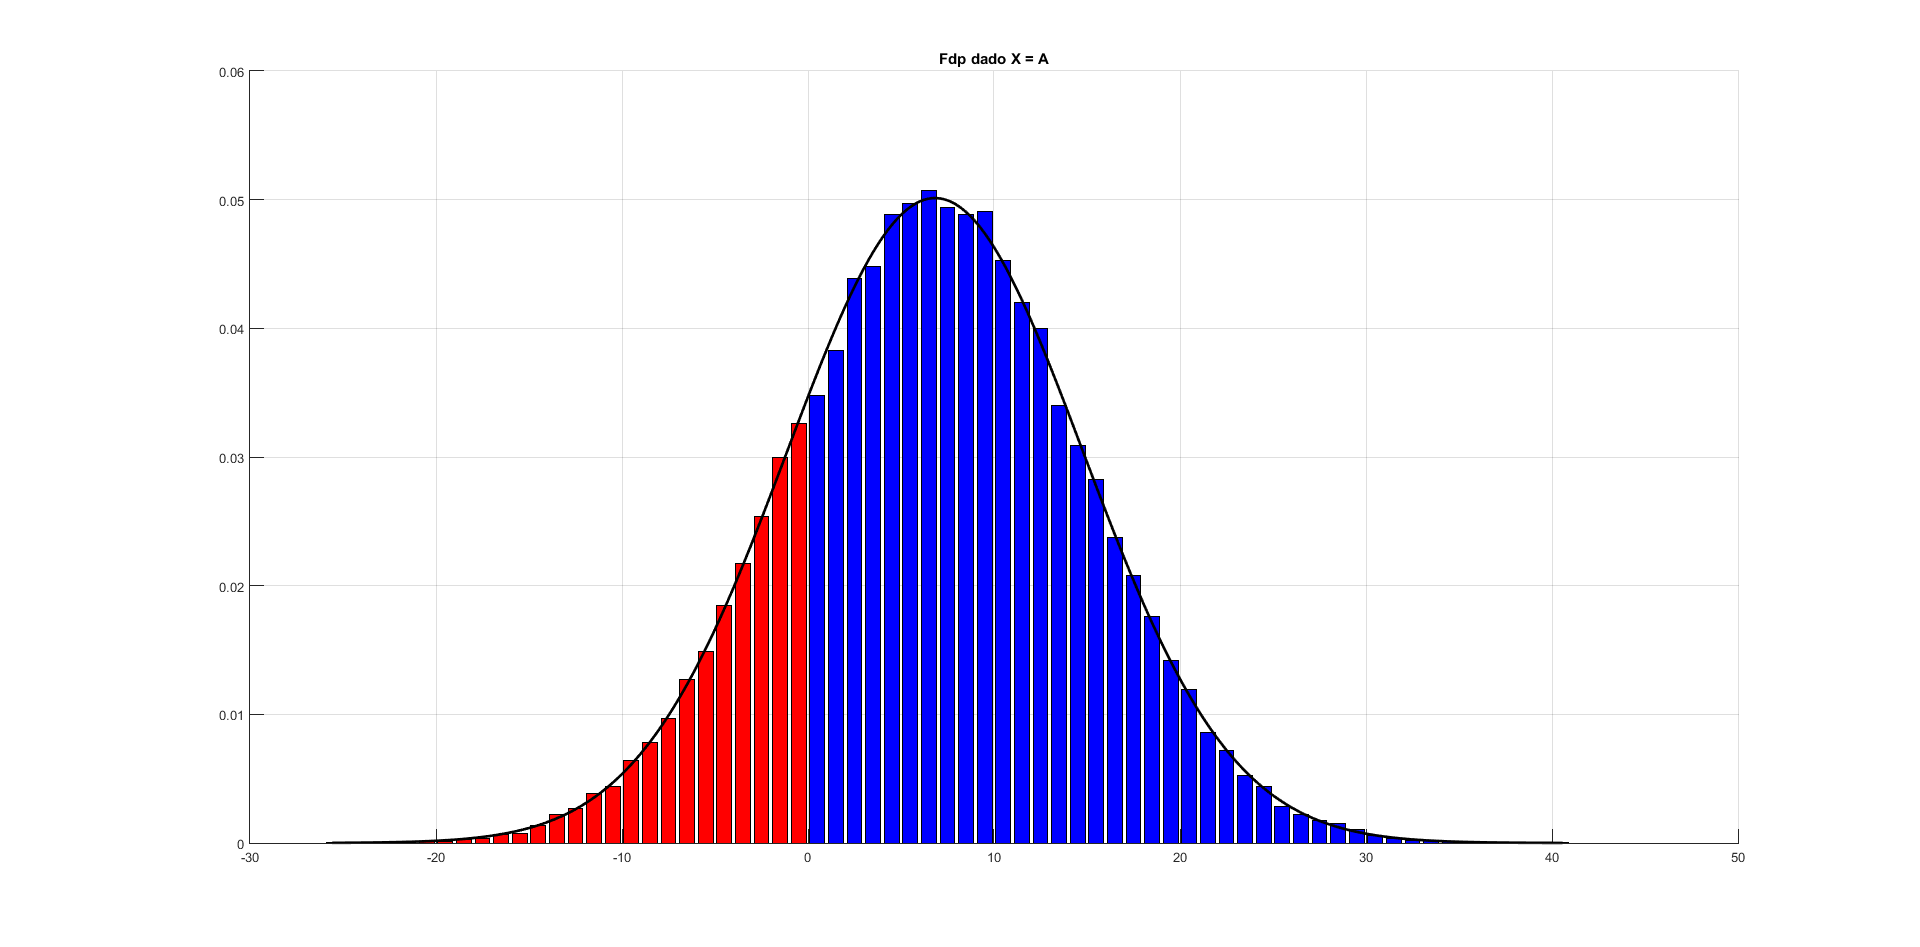
\includegraphics[width=1\textwidth]{images/fdp_XA}
  \caption{Función de densidad de probabilidad $f_{Y_n|X=A}$. En rojo los eventos de Error.}
  \label{fig:pto4_3}
\end{figure}	

\begin{figure}[H]
  \centering
  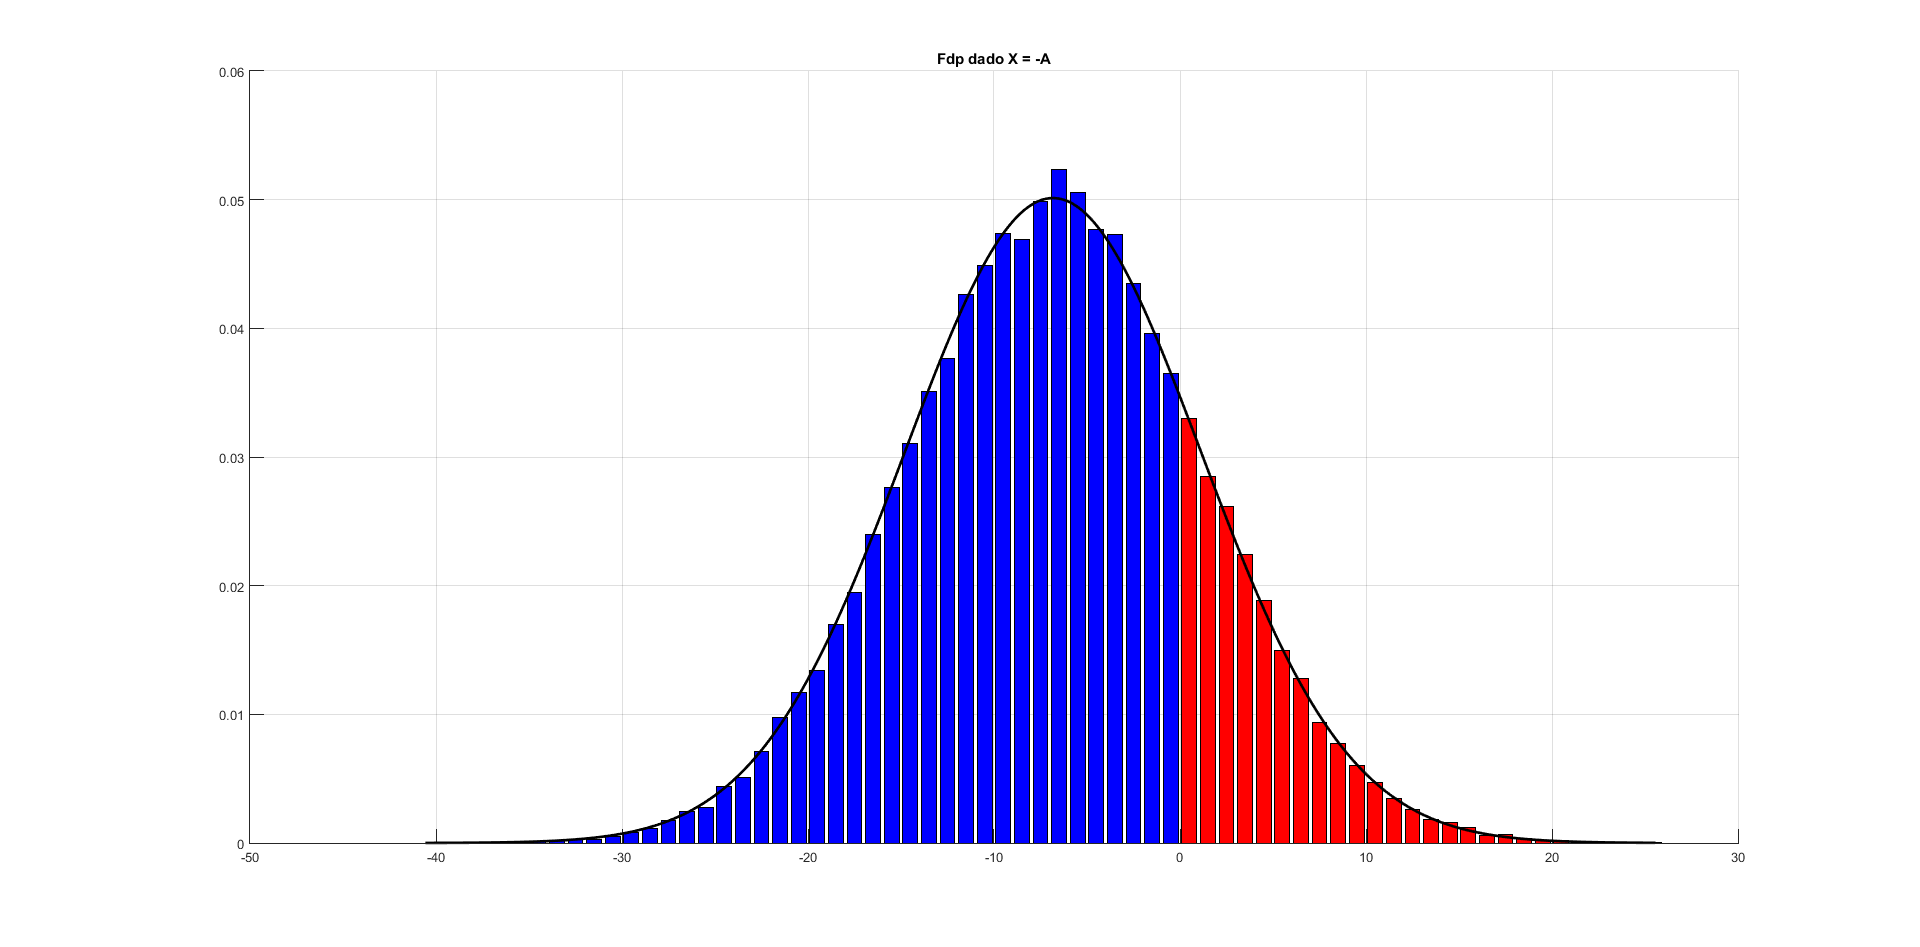
\includegraphics[width=1\textwidth]{images/fdp_X-A}
  \caption{Función de densidad de probabilidad $f_{Y_n|X=-A}$. En rojo los eventos de Error.}
  \label{fig:pto4_3b}
\end{figure}
























\newpage
\section{Conclusiones}
\label{sec:conclu}

Como conclusión podemos decir que es muy sencillo diseñar un sistema de repetidores tanto digital como analógico utilizando la herramienta de calculo correspondiente para poder conocer sus alcances y falencias.

Más importante aún por medio de las simulaciones tenemos información más certera sobre las hipótesis teóricas calculadas previamente.  

En particular notamos que a medida que aumenta la relación de señal ruido SNR, mejora más rápido el sistema digital comparado al analógico. 

Sin embargo la señal analógica con ruido puede ser interpretada por un ser humano, de modo que la información transmitida puede llegar al receptor aún con ruido.
En cambio la señal digital no posee ninguna distorsión sino que su funcionamiento es binario, se interpreta la información transmitida o no.
%\section{Apéndice}
%\label{sec:apend}







\end{document}


